%
% band.tex -- Karten eines Bandes
%
% (c) 2021 Prof Dr Andreas Müller, OST Ostschweizer Fachhochschule
%
\documentclass[tikz]{standalone}
\usepackage{amsmath}
\usepackage{times}
\usepackage{txfonts}
\usepackage{pgfplots}
\usepackage{csvsimple}
\usetikzlibrary{arrows,intersections,math}
\begin{document}
\def\skala{1}
\def\l{1}
\def\u{0.89}
\definecolor{farbenull}{rgb}{1.0,0.6,0.8}
\definecolor{farbeeins}{rgb}{0.8,1.0,0.6}
\definecolor{farbezwei}{rgb}{0.6,0.8,1.0}
\definecolor{darkred}{rgb}{0.8,0,0}
\definecolor{darkgreen}{rgb}{0,0.6,0}
\begin{tikzpicture}[>=latex,thick,scale=\skala]
\clip (-0.9,-7.63) rectangle ++(12.5,15.5);

\begin{scope}[yshift=5cm]
	\node at ({6*\u},0) {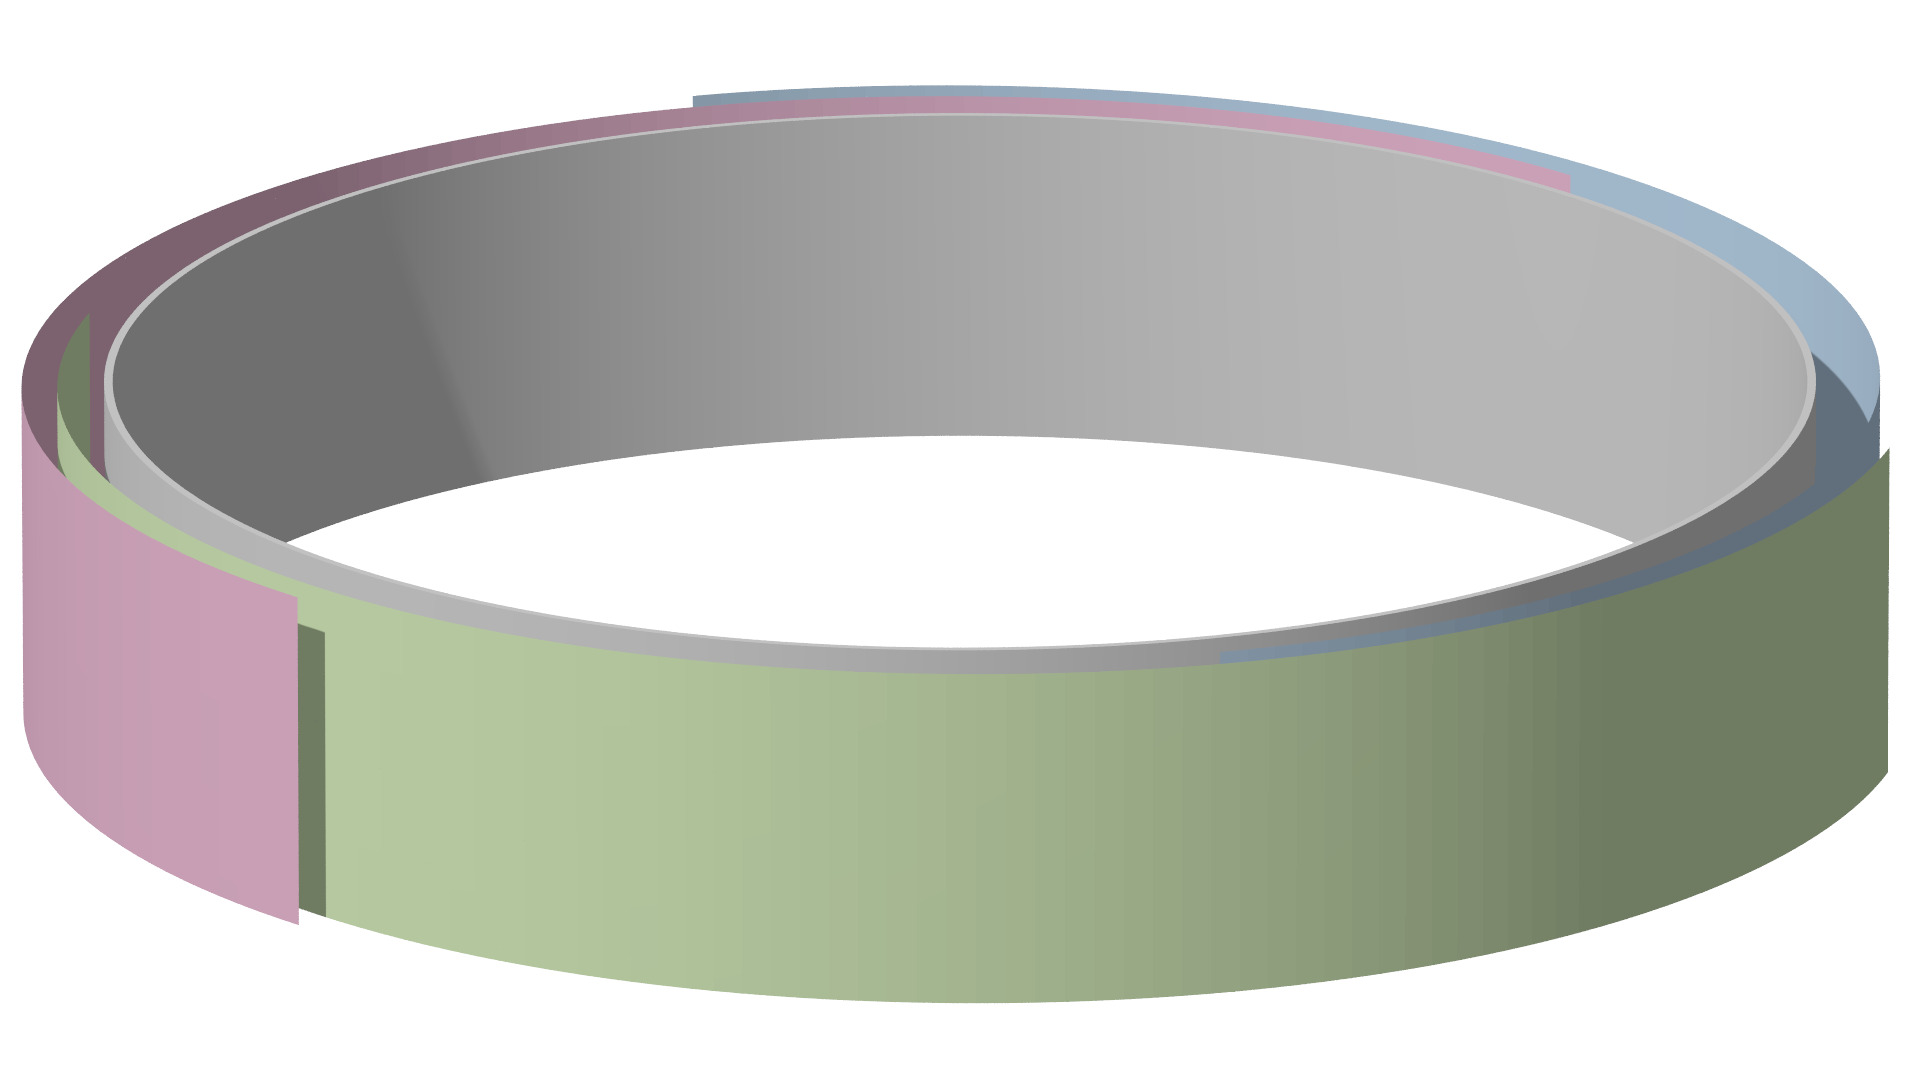
\includegraphics[width=12cm]{band.jpg}};
	\node at ({6*\u},1.7) {$M$};
	\node[color=darkred] at (0.4,-1.1) {$U_0$};
	\draw[->,color=darkred] (0.4,-2.2) to[out=-110,in=135]  ++(1,-1.7);
	\node[color=darkred] at (0.4,-3.2) {$\varphi_0$};

	\node[color=darkgreen] at ({6*\u},-1.9) {$U_1$};
	\draw[->,color=darkgreen] ({6*\u},-3.0) -- ++(0,-3.4);
	\node[color=darkgreen] at ({6*\u},-4.8) [right] {$\varphi_1$};

	\node[color=blue] at ({12*\u},2) {$U_2$};
	\node[color=blue] at ({11*\u+0.1},-7) {$\varphi_2$};
	\draw[->,color=blue] ({12.6*\u},0) to[out=-60,in=90]
	({13*\u},-1.5) to[out=-90,in=60] ({10*\u},-9.4);
\end{scope}

\fill[color=farbenull!50] ({-\u},-\l) rectangle ({5*\u},\l);
\fill[color=gray!20,opacity=0.5] ({-\u},-\l) rectangle ({\u},\l);
\fill[color=gray!20,opacity=0.5] ({3*\u},-\l) rectangle ({5*\u},\l);
\draw (-\u,-\l) rectangle ({5*\u},\l);
\node at ({2*\u},\l) [above] {$V_0$};
\node at ({4*\u},0) {$\varphi_0(U_0\cap U_1)$};

\begin{scope}[yshift=-3cm]
	\fill[color=farbeeins!50] ({3*\u},-\l) rectangle ({9*\u},\l);
	\fill[color=gray!20,opacity=0.5] ({3*\u},-\l) rectangle ({5*\u},\l);
	\fill[color=gray!20,opacity=0.5] ({7*\u},-\l) rectangle ({9*\u},\l);
	\draw ({3*\u},-\l) rectangle ({9*\u},\l);
	\node at ({6*\u},\l) [above] {$V_1$};
	\node at ({8*\u},0) {$\varphi_1(U_1\cap U_2)$};
	
\end{scope}

\begin{scope}[yshift=-6cm]
	\fill[color=farbezwei!50] ({7*\u},-\l) rectangle ({13*\u},\l);
	\fill[color=gray!20,opacity=0.5] ({7*\u},-\l) rectangle ({9*\u},\l);
	\fill[color=gray!20,opacity=0.5] ({11*\u},-\l) rectangle ({13*\u},\l);
	\draw ({7*\u},-\l) rectangle ({13*\u},\l);
	\node at ({10*\u},\l) [above] {$V_2$};
	\node at ({12*\u},0) {$\varphi_2(U_2\cap U_0)$};
\end{scope}

\draw[->] ({4*\u},{-\l+0.3}) -- ++(0,-1.6);
\node at ({4*\u},{-\l-0.5}) [right] {$\psi_{01}$};

\begin{scope}[yshift=-3cm]
	\draw[->] ({8*\u},{-\l+0.3}) -- ++(0,-1.6);
	\node at ({8*\u},{-\l-0.5}) [right] {$\psi_{12}$};
\end{scope}

\begin{scope}[yshift=-6cm]
	\draw[->] ({12*\u},{-\l+0.3})
		-- ++(0,-0.6)
		to[out=-90,in=0] ++(-0.3,-0.3)
		-- ++({-12*\u+0.6},0)
		to[out=180,in=-90] ++(-0.3,0.3)
		-- ++(0,6.6);
	\node at (0,1) [right] {$\psi_{20}$};
\end{scope}

\end{tikzpicture}
\end{document}

